\newpage
\section{Functional Requirements}
    \label{section:functionalReq}
    This section describes the functional requirements for the Archive service.
    The requirements mentioned here are the expected benchmarks for the designed system which are also depicted in Figure \ref{fig:archiveUseCase}.
    The functional aspects which carves the Archive service are mentioned below.

    \subsection{Archive project resources}
        The designed system should be able to archive the MARS resources from the active system (Ceph cluster at the time of writing) 
        into the Synology \cite{Synology}. The application should
        be able to archive a project even when there all the MARS resources are not present in the project (e.g. no simulation runs have been triggered).
        This should be supported since it could be the case that the user wants to archive only some of the resources. The resources which are to be archived
        are depicted in a tabular format (Table \ref{table: archivedMars}).
        
        \begin{table}[h!]
            \centering
            \begin{tabular}{|p{3cm}|p{12cm}|}
                \hline
                    \textbf{Resource Name}  & \textbf{Description}\\
                \hline
                     Metadata & 
                     This resource stores the metadata (e.g. file id, file name). It gives the system the information about
                     existing files in the system. \\
                \hline
                     Files & 
                     This resource correspond to the models and files which describe a simulation (e.g. wolves and sheep model). \\
                \hline
                     Scenario & 
                     This resource defines the parameters for the model which would be simulated (e.g. simulation run time, number of agents). \\
                \hline
                     Result configurations & 
                     This resource maps which agents in the simulation are present in the simulation run.\\
                \hline
                     Simulation plan & 
                     This resource contains the scenario and the result configuration which can be executed. The simulation plan could be configured to
                     have different scenario and result configuration to produce different kind of output.\\
                \hline
                     Simulation run & 
                     This resource contains the metadata for a simulation results i.e. simulation id, simulation status.\\
                \hline
                     Simulation result & 
                     This resource is the output and contains the results for a single simulation run.\\
                \hline
            \end{tabular}
            \caption{MARS resources which are to be archived}
            \label{table: archivedMars}     
        \end{table} 

        The resources depicted in table (Table \ref{table: archivedMars}) must be archived following the MARS resource hierarchy (Figure \ref{fig:marsDependency}).
        Following the hierarchy, it is arguable why the project is not being archived, despite it being present. Due to the fact that retrieving the project is also 
        desired and it is connected to multiple users which may not exist in the future. To avoid complexity of dealing with many users, the project is
        not archived. 
        \subsubsection{Assurance of correct data being persisted}
            MARS being a Distributed System, Data Coherency (Subsection \ref{subsection: distriChallenges}) 
            is one of the big issue which this thesis faces. As a consequence,
            wrong or unwanted data could be archived. To avoid this the Archive service should include some kind of mechanism that
            could lock the MARS resources during the archive process.
        
        \subsection{Retrieve project resources}    
            The designed software should support the retrieval of the archived projects from the Synology into the active system. The
            system should be able to restore the project given that, the services support the data format which is archived in the Synology.
           
            \begin{figure}[H]
                \centering 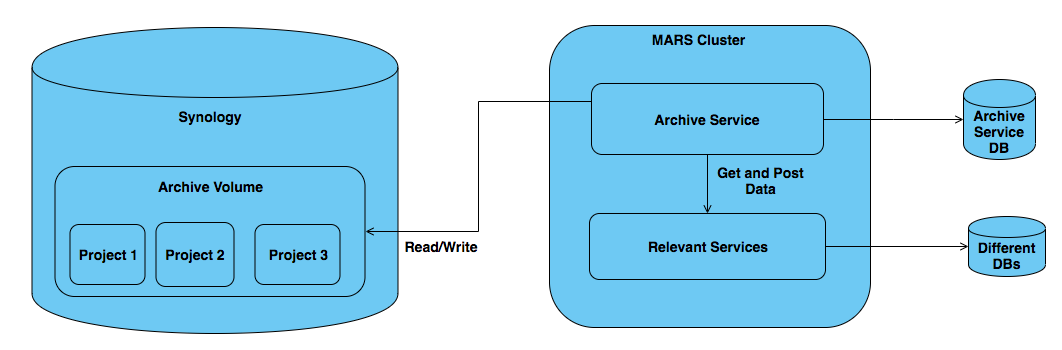
\includegraphics[scale=0.4]{grafiken/synology.png}
                \caption{Archive service's communication structure}
                \label{fig:synology}
            \end{figure}

            Figure \ref{fig:synology} illustrates the communication procedure required to be implemented for the archive and retrieval process. 
            This requirement must be fulfilled to comply with the MARS development standard. As seen, the
            Archive service can read and write directly only to the archive volume in Synology and its own database. The data which is not owned by the archive
            service has to be requested via an API to the relevant service for read/write purposes. The figure generalizes the services it communicates with
            as "Relevant Services" because this diagram only intends to show an abstraction for the communication between them.


        \subsection{Archive and retrieve process status}  
            The archive and retrieve processes are a long running tasks. The designed software must run these processes in the background to avoid 
            long waiting time for another request. Given this, a API endpoint should be made available which gives the current status of the archive 
            or retrieve job. Using the status a user can determine whether the job is being executed or is finished.


        \subsection{Download archived data as a compressed file}
            It is of great importance for a Domain Expert i.e. ecologist who are not technical experts to have a graphical interface in hand. In this interface
            it should be possible to navigate to the project of interest and easily download the project as a zip file. There could be cases where the
            MARS system is out of order and the data is required which could then be accessible by anyone with basic knowledge of the system.
        
        \subsection{Design for Failure}   
        Firstly, the Archive service has to communicate with many services in the system, leading the rate of failure being higher
        in comparison to a system which does not depend on other services. A breakdown 
        of one service would cause the whole process of archive/retrieve to stop unexpectedly.  Secondly, it is also possible that a running Archive service be terminated
        due to some unexpected reason. Therefore, fault tolerance mechanism has to be included in the Archive system so that it has a chance of 
        recovery. 
